% !TXS template
\documentclass[titlepage]{article}
\usepackage[utf8]{inputenc}
\usepackage{color}   %May be necessary if you want to color links
\usepackage{hyperref}
\usepackage[french]{babel}
\usepackage{cite}
\usepackage{graphicx}

\hypersetup{
	colorlinks=true, %set true if you want colored links
	linktoc=all,     %set to all if you want both sections and subsections linked
	linkcolor=blue,  %choose some color if you want links to stand out
}
\title{Arbre comportementaux pour le contr\^ole de mission}
\author{
	Derrien Martial \\
	\and
	Madec Antoine \\
	\and
	Lucas Florian
}
\date{Juin 2019}
\renewcommand{\contentsname}{Sommaire} 
\begin{document}
	\maketitle
	\tableofcontents
	\hypersetup{linktocpage}
	
	\clearpage
	\part{Introduction}
	Un arbre comportemental (Behavior Tree, BT en anglais) est une
	technique permettant de structurer le passage d'une tâche à une autre dans 
	le cadre de l'automatisation de ce comportement.
	\\
	\begin{figure}[h!]
		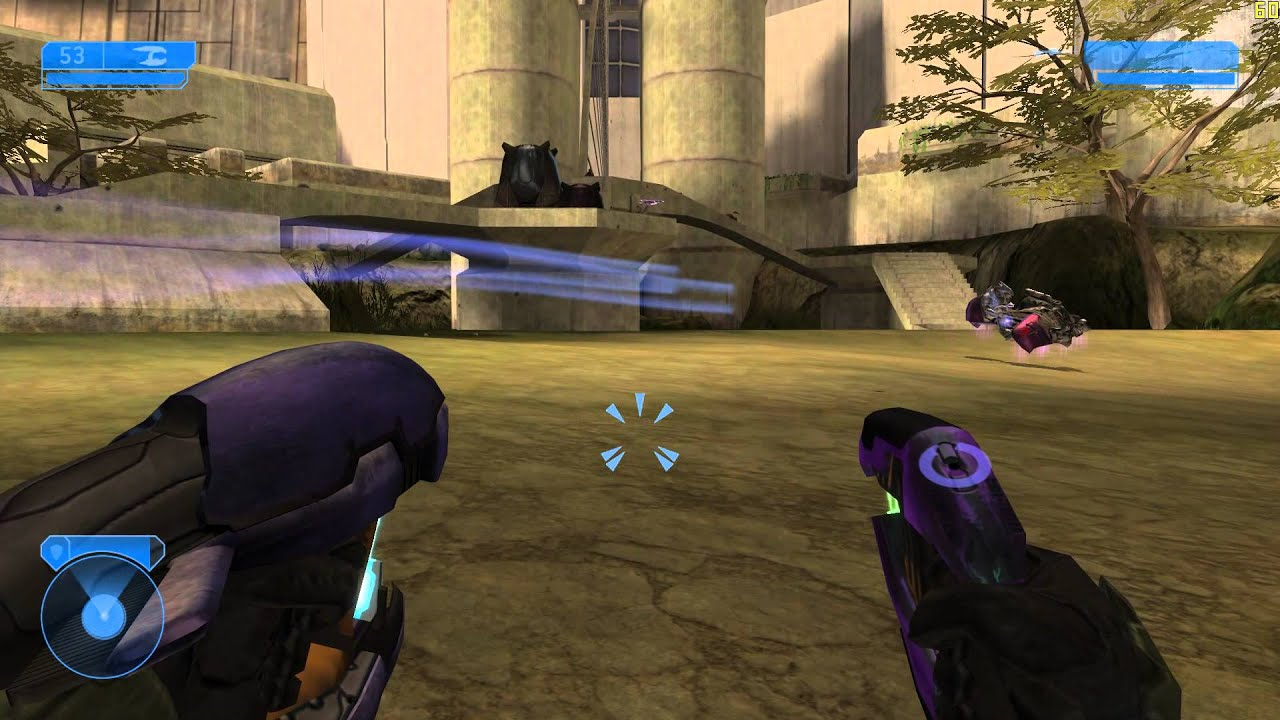
\includegraphics[width=\linewidth]{img/halo2.jpg}
		\caption{Le jeu vidéo Halo2, un précurseur en matière d'intelligence artificielle dans le jeu vidéo grâce à son utilisation des BT \cite{wikipedia_halo}}
		\label{fig:BT1}
	\end{figure}
	\\
	Cette technique, d'abord utilisé pour programmer le comportement de personnages non joueurs (NPC) dans les jeux vidéos \cite{wikipedia_BT}, est maintenant l'une des techniques les plus en vogue pour la programmation de robot autonome ou semi-autonome\cite{ros.org}.
	\\
	photo robot thalès ? 
	\\
	Le but de ce rapport est de faire une synthèse de l'utilisation émergente des BT en robotique pour mener à bien des missions, et ce dans plusieurs domaines.
	
	\clearpage
	\part{Qu'est-ce-qu'un behavior tree ?}
	todo
	\\
	\begin{figure}[h!]
		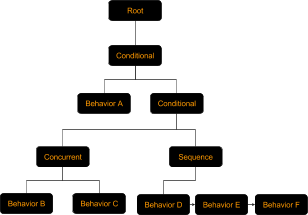
\includegraphics[width=\linewidth]{img/behavior_trees_example.png}
		\caption{exemple de BT \cite{rasmussen}}
		\label{fig:BT1}
	\end{figure}
	\\
	
	\clearpage
	\part{Les grands domaines d'emploi des behavior trees}
	\section{civil}
	
	\section{industrie}
	
	\section{santé}
	prédire comportement
	
	\section{militaire}
	prédire comptmt
	
	\clearpage
	\part{Les outils utilisés dans la mise en place des behavior trees}
	\section{machine learning}
	
	\clearpage
	\part{Exemple de behavior tree}
	
	\clearpage
	\bibliographystyle{alpha}
	\bibliography{sources.bib}
	
\end{document}
